\subsection{Estudos de Regressão}

Ao montarmos a visualização dos tempos de chegada ao longo do tempo percebemos que havia tendência nos dados. Para isso, primeiro, calculamos todos os tempos de chegada das chamadas, subtraindo o horário de recebimento de uma chamada subsequente pelo da anterior, isto é:

$$Tempo_{chegada}(c_n) = t_n - t_{n-1}$$ 

\begin{itemize}
    \item $c_n$ é a chamada de número $n$
    \item $t_n$ é o tempo de recebimento da chamada $n$
    \item $t_{n-1}$ é o tempo de recebimento da chamada $n-1$
\end{itemize}

Depois, as chamadas foram classificadas por dia, e, assim, calculado o tempo de chegada médio diário delas. O principal intuito desta etapa é facilitar a visualização da evolução desse parâmetro ao longo do tempo. O gráfico obtido por essa operação está abaixo.

\begin{figure}[H]
    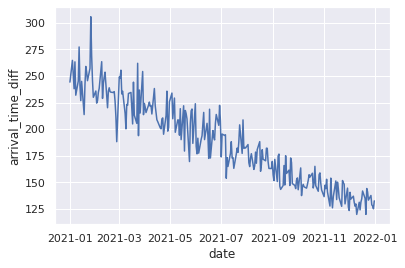
\includegraphics{analise-de-dados/regressao/tempo_chegada_medio.png}
    \caption{Tempo médio de chegada ao longo do Ano}
    \label{fig: tempos_de_chegada}
\end{figure}

A partir dessa percepção, são, então, propostos alguns estudos de regressão mais particulares para representar a tendência dos dados. Um usando "Ordinary Least Squares", outro usando "Generalized Least Squares" e uma regressão exponencial.  